\documentclass[11pt]{article}
\usepackage[margin=1.1in]{geometry}
\usepackage{amsmath,amssymb,amsthm}
\usepackage[round]{natbib}
\usepackage{graphicx}
\usepackage{hyperref}
\hypersetup{hidelinks}
\usepackage{microtype}

\newtheorem{theorem}{Theorem}
\newtheorem{proposition}[theorem]{Proposition}
\newtheorem{lemma}[theorem]{Lemma}
\newtheorem{corollary}[theorem]{Corollary}
\theoremstyle{definition}
\newtheorem{definition}[theorem]{Definition}
\newtheorem{assumption}{Assumption}
\theoremstyle{remark}
\newtheorem{remark}[theorem]{Remark}

\newcommand{\R}{\mathbb{R}}
\newcommand{\E}{\mathbb{E}}
\newcommand{\Prob}{\mathbb{P}}
\newcommand{\KL}{D_{\mathrm{KL}}}
\newcommand{\TV}{\mathrm{TV}}
\newcommand{\Hs}[1][s]{\mathcal{H}^{#1}}
\newcommand{\given}{\,|\,}

\title{Locally Honest Coverage Forces Nonparametric Inflation:\\
a Sharpness Lower Bound for Prediction Sets}
\author{Peter Cotton\\\texttt{peter.cotton@microprediction.com}}
\date{August 2026}

\begin{document}
\maketitle

\begin{abstract}
Marginal conformal coverage is compatible with oracle-rate sharpness and does not impose
the bound studied here. A guarantee at a fixed test point is different. We show that any
honestly valid procedure must, at a fixed smooth baseline, exceed the oracle threshold by
the local modulus $(n g(x_0))^{-s/(2s+d)}$ on a majority of samples. The cause is Le~Cam
indistinguishability, a testing-power floor, not exchangeability. For fixed $\eta>0$,
minimax-rate sharpness stays compatible with honesty. Zero excess and adaptation to unknown
smoothness are not. A plug-in estimate can be sharper because it declines to insure against
alternatives the data cannot rule out.
\end{abstract}

\section{Two guarantees, one honest}

Fix a model, freeze it, and let $R = A(X,Y)$ be its scalar nonconformity score with
conditional law $\mathcal{L}(R\given X=x)$. Ordinary conformal coverage is
\begin{equation}\label{eq:marginal}
  \Prob\big\{ R_{n+1} \in C_n(X_{n+1}) \big\} \;\ge\; 1-\alpha ,
\end{equation}
the probability averaging over the test point $X_{n+1}$ and the calibration sample $D_n$.
The honesty lower bound below does not follow from marginal validity:
\citet{lei2014distribution} construct bands with exact finite-sample marginal validity that
converge to an oracle band at the minimax rate, and localized conformal methods retain
marginal validity while weighting by proximity. The cost we identify attaches not to
marginal coverage but to a guarantee at a fixed point, formalized next as honest local
coverage.

\begin{definition}[Honest local coverage]\label{def:honest}
Fix an interior point $x_0$ and $0 \le \eta < \tfrac12$. A one-sided prediction set
$C_n(x_0) = [0, T_n(x_0)]$ for a nonnegative score is \emph{honestly locally valid} over a
class $\Theta$ if
\begin{equation}\label{eq:honest}
  \inf_{\theta \in \Theta}\;
  \Prob_{\theta}\!\Big\{ F_{\theta(x_0)}\big(T_n(x_0)\big) \ge 1-\alpha \Big\}
  \;\ge\; 1-\eta ,
\end{equation}
where $F_{\theta(x_0)}$, assumed continuous and strictly increasing, is the true
conditional law of the score at $x_0$, so the event equals
$\{T_n(x_0)\ge q_\alpha(\theta(x_0))\}$, and the probability is over the calibration
sample. In words: with probability at least $1-\eta$
over the data, the realized set has conditional coverage $1-\alpha$ at $x_0$, whatever
law in $\Theta$ generated the data. Taking $\eta=0$ asks for coverage almost surely over
the calibration sample. This is a training-conditional, fixed-$x_0$ requirement, the local
analogue of the training-conditional and tolerance-region guarantees studied for conformal
sets \citep{vovk2012conditional}, and it is deliberately stronger than the marginal coverage
\eqref{eq:marginal}.\footnote{\emph{Honesty} refers to coverage uniformly over the model
class, the $\inf_\theta$ sitting inside the probability, as opposed to a pointwise guarantee
that fixes $\theta$ first \citep{li1989honest,low1997nonparametric,cai2004adaptation}. It is
often stated asymptotically. Here we impose the stronger nonasymptotic version at every $n$.
And \emph{local} means the requirement is imposed at the fixed point $x_0$ rather than over
an interval.}
\end{definition}

Sharpness is measured against the oracle threshold $q_\alpha(u) = F_u^{-1}(1-\alpha)$
through the excess
\begin{equation}\label{eq:sharp}
  S_\theta(T_n) \;=\; \E_\theta\Big[\big(T_n(x_0) - q_\alpha(\theta(x_0))\big)_{+}\Big] ,
\end{equation}
the expected inflation of the threshold above the oracle. The question is how small
\eqref{eq:sharp} can be made subject to \eqref{eq:honest}.

\section{Assumptions}

The upper H\"older bound alone is not enough for a lower bound. The class must contain
alternatives that are indistinguishable near $x_0$. Three standing assumptions supply this
without asking us to estimate an arbitrary law.

\begin{assumption}[Local design regularity]\label{as:design}
The covariate density $g$ satisfies $0 < g_- \le g(x) \le g_+ < \infty$ on a fixed
neighbourhood of $x_0 \in (0,1)^d$, and $x_0$ is a Lebesgue point of $g$.
\end{assumption}

All the proof uses is the local-averaging relation, valid at a Lebesgue point of $g$,
\[
  \int \psi^2\!\Big(\frac{x-x_0}{h}\Big)\,g(x)\,dx
    \;=\; h^{d}\,g(x_0)\!\int\!\psi^2(z)\,dz \;+\; o(h^d),
\]
which turns the bump support into $\asymp n\,g(x_0)\,h^{d}$ effective observations. The same
relation holds on smooth manifolds and under non-Euclidean metrics, with $g(x_0)$ the local
density and $d$ the intrinsic dimension. Without the Lebesgue point the local mass is only
pinned between constants times $h^d$, and every rate below holds with $g(x_0)$ replaced by a
constant in $[g_-,g_+]$. Boundaries and sparse high-dimensional regions violate the
assumption and need separate treatment.

\begin{assumption}[Regular one-dimensional residual submodel]\label{as:family}
The calibration sample $(X_i,R_i)_{i=1}^n$ is i.i.d.\ with $X_i\sim g$, and the admissible
class of conditional score laws contains a one-parameter submodel
$R \given X=x \sim F_{\theta(x)}$, $\{F_u : u \in [\underline u, \overline u]\}$, that is,
locally in $u$, quadratically regular in information and Lipschitz-regular in quantile:
\[
  \KL\big(F_u \,\|\, F_v\big) \le K\,(u-v)^2,
  \qquad
  c_q\,|u-v| \le \big|q_\alpha(u) - q_\alpha(v)\big| \le C_q\,|u-v| .
\]
The lower bound needs only the quadratic information bound and the lower quantile constant
$c_q$. The upper constant $C_q$ enters only attainability (Section~\ref{sec:attain}).
\end{assumption}

The submodel framing is the point. Even if the true residual law varies in scale,
skewness, and tail thickness, the impossibility follows as soon as the class contains
\emph{one} regular direction that moves the target quantile, and a lower bound proved on
the submodel applies to every larger class containing it. In a smooth dominated family for
which the usual local Kullback--Leibler expansion holds, uniformly bounded Fisher
information yields the quadratic information bound. If $q_\alpha$ is continuously
differentiable with $0<c\le q_\alpha'(u)\le C$, the quantile inequalities follow by the
mean-value theorem. The two-sided quantile bound forces $q_\alpha$ strictly monotone, so we
orient the parameter to make it increasing. What is excluded is worth naming: discrete
scores, quantiles in flat parts of a CDF, parameters with $q_\alpha'(u)=0$, and families
with parameter-dependent support giving infinite $\KL$.

Three standard scores satisfy the submodel exactly on a compact parameter interval
$[\underline u,\overline u]$, with $z_p=\Phi^{-1}(p)$ and $c_\alpha =
F^{-1}_{\chi^2_1}(1-\alpha)$.
\begin{itemize}
\item[(A)] \emph{Heteroskedastic squared-Gaussian score.} $E\given X=x \sim N(0,e^{2u})$,
  $R=E^2 \sim e^{2u}\chi^2_1$. Then $q_\alpha(u)=c_\alpha e^{2u}$ and
  $\KL(F_u\|F_v)=\tfrac12[e^{2(u-v)}-1-2(u-v)] \le e^{2\rho}(u-v)^2$ for $|u-v|\le\rho$. The
  result therefore already applies to ordinary heteroskedastic Gaussian errors and squared
  residuals.
\item[(B)] \emph{Lognormal positive score.} $R=\exp\{u+\sigma Z\}$, $Z\sim N(0,1)$. Then
  $\KL(F_u\|F_v)=(u-v)^2/(2\sigma^2)$ exactly and $q_\alpha(u)=\exp\{u+\sigma z_{1-\alpha}\}$,
  so both bounds hold with $c_q=e^{\underline u+\sigma z_{1-\alpha}}$,
  $C_q=e^{\overline u+\sigma z_{1-\alpha}}$. This model gives a rigorous attainability
  construction (Section~\ref{sec:attain}) and the exact numerical check (Section~\ref{sec:check}).
\item[(C)] \emph{Exponential scale.} $R\given u \sim \mathrm{Exp}(\text{mean }e^{u})$. Then
  $\KL(F_u\|F_v)=e^{u-v}-1-(u-v)$ and $q_\alpha(u)=-(\log\alpha)e^{u}$. Both bounds follow
  on a compact interval, with no truncation needed.
\end{itemize}

\begin{assumption}[H\"older smoothness with local richness]\label{as:holder}
Write $k=\lceil s\rceil-1$ and $\gamma=s-k\in(0,1]$, so $s=k+\gamma$ with the Lipschitz
class $s=1$ giving $k=0,\gamma=1$, and let $\Hs(L)$ be the ball of fields $\theta$ with
$k$th derivatives $\gamma$-H\"older with seminorm $\le L$ and range
$\theta(x)\in[\underline u,\overline u]$. Fix a bump profile $\psi$ with $\psi(0)=1$,
$\|\psi\|_\infty\le1$, $\operatorname{supp}\psi \subseteq B(0,1)$, and $\psi\in C^s$. There
are $h_0,a_0>0$ and an interior baseline value $u_0\in(\underline u,\overline u)$ with
\[
  \theta_{h,a}(x) = u_0 + a\,L\,h^{s}\,\psi\!\Big(\frac{x-x_0}{h}\Big) \in \Hs(L),
  \qquad 0<h<h_0,\ \ 0<a<a_0 .
\]
The scaling $a L h^{s}\psi((x-x_0)/h)$ has $C^s$ seminorm $\asymp a L$ independent of $h$,
so small $a$ keeps it in the ball.
\end{assumption}

Assumption~\ref{as:holder} is the operative one, and it is not innocuous. It holds for
broad H\"older classes that permit localized features at the detection boundary. Global
parametric structure, analyticity, monotonicity, or self-similarity may exclude the local
bump alternatives, and under additional conditions can change or restore the adaptation
problem. Within a H\"older
ball it says the class holds a pair that agree outside a ball of radius $h$ around $x_0$ but
differ by $\delta = a L h^{s}$ at $x_0$, with the amplitude $a$ shrinkable below $a_0$,
which the proof uses to place the two hypotheses at any chosen separation.

\section{The lower bound}

The bound is at bottom a testing-power statement, so we isolate that step. For laws
$P_1,P_0$ on the calibration sample write the Neyman--Pearson frontier
\begin{equation}\label{eq:frontier}
  \beta_{1-\eta}(P_1,P_0) \;=\; \inf_{A:\,P_1(A)\ge 1-\eta} P_0(A) ,
\end{equation}
the least $P_0$-mass of any event whose $P_1$-mass is at least $1-\eta$.

\begin{lemma}[Honesty is a test, and a test has a floor]\label{lem:test}
Let $\theta_0,\theta_1$ be two parameter fields with $q_1 := q_\alpha(\theta_1(x_0)) >
q_\alpha(\theta_0(x_0)) =: q_0$, and let $T_n$ satisfy honest local coverage
\eqref{eq:honest} under $\theta_1$. Then
\[
  \Prob_{\theta_0}\big\{ T_n(x_0) \ge q_1 \big\}
    \;\ge\; \beta_{1-\eta}\big(P^n_{\theta_1},P^n_{\theta_0}\big) ,
  \qquad
  S_{\theta_0}(T_n) \;\ge\; (q_1-q_0)\,
    \beta_{1-\eta}\big(P^n_{\theta_1},P^n_{\theta_0}\big) .
\]
\end{lemma}

\begin{proof}
Honesty under $\theta_1$ makes $A=\{T_n(x_0)\ge q_1\}$, a function of the calibration
sample, satisfy $P^n_{\theta_1}(A)\ge 1-\eta$, so $P^n_{\theta_0}(A)\ge\beta_{1-\eta}$ by
\eqref{eq:frontier}. On $A$ the excess $T_n(x_0)-q_0$ is at least $q_1-q_0$, giving the
second inequality. The frontier obeys the Le Cam bound
$\beta_{1-\eta}(P_1,P_0)\ge 1-\eta-\TV(P_1,P_0)$, since any $A$ with $P_1(A)\ge1-\eta$ has
$P_0(A)\ge P_1(A)-\TV$.
\end{proof}

The frontier \eqref{eq:frontier} is exact, and the $1-\eta-\TV$ reading is the crude corollary.
Both feed the same conclusion once the two hypotheses are placed at critical separation.

\begin{theorem}[Honest local coverage forces inflation]\label{thm:main}
Fix $0<\alpha<1$ and $0 \le \eta < \tfrac12$, and let
Assumptions~\ref{as:design}--\ref{as:holder} hold. There are constants $c_1,c_2>0$ and
$n_0$, depending on the fixed model class $(s,d,L,\alpha,\eta,K,c_q)$, the local design law
$g$ near $x_0$, and the bump profile $\psi$, but not on $n$, and a fixed constant baseline
$\theta_0\in\Hs(L)$, such that for all $n\ge n_0$ every $T_n$ satisfying
honest local coverage \eqref{eq:honest} over $\Hs(L)$ has, with
$r_n := L^{d/(2s+d)}\big(n\,g(x_0)\big)^{-s/(2s+d)}$,
\begin{equation}\label{eq:tail}
  \Prob_{\theta_0}\big\{\, T_n(x_0) - q_\alpha(\theta_0(x_0)) \;\ge\; c_1\,r_n \,\big\}
  \;\ge\; c_2 \;>\; \tfrac12 .
\end{equation}
In particular the realized threshold exceeds the oracle by order $r_n$ on a majority of
samples, so both its median excess and its expected positive excess satisfy
\begin{equation}\label{eq:rate}
  \sup_{\theta \in \Hs(L)} S_\theta(T_n)
  \;\ge\; S_{\theta_0}(T_n) \;\ge\; c_1 c_2\, r_n .
\end{equation}
\end{theorem}

\begin{proof}
Take the constant baseline $\theta_0 \equiv u_0$ and the bump $\theta_1=\theta_{h,a}$ of
Assumption~\ref{as:holder}. Since $\psi(0)=1$ and $q_\alpha$ is oriented increasing
(Assumption~\ref{as:family}), $q_1=q_\alpha(u_0+\delta)>q_\alpha(u_0)=q_0$. If $\psi(0)=1$
gave a decrease we would flip the sign of $\psi$. Both fields lie in $\Hs(L)$.

\emph{Indistinguishability.} The two laws differ only on the bump support, of covariate
measure $g(x_0)h^{d}(1+o(1))$ by Assumption~\ref{as:design}. Integrating the per-point
divergence bound $\KL(F_{\theta_1(x)}\|F_{u_0})\le K\delta^2\psi((x-x_0)/h)^2$ of
Assumption~\ref{as:family} against the i.i.d.\ sample,
\[
  \KL\big(P^{n}_{\theta_1} \,\|\, P^{n}_{\theta_0}\big)
  \;\le\; n\,K\,a^2 L^2 h^{2s+d}\,g(x_0)\!\int\!\psi(z)^2\,dz\,(1+o(1)),
  \qquad \delta = a\,L\,h^{s}.
\]
Fix the bandwidth by $h = c_h\big(L^2 n g(x_0)\big)^{-1/(2s+d)}$. The divergence bound
becomes $K a^2 c_h^{2s+d}\|\psi\|_2^2(1+o(1))$, free of $n$, and the quantile shift is
\[
  q_1 - q_0 \;\ge\; c_q\,\delta \;=\; c_q\,a\,L\,h^{s}
    \;=\; c_q\,a\,c_h^{s}\,L^{d/(2s+d)}\big(n g(x_0)\big)^{-s/(2s+d)}
    \;=\; c_1\,r_n ,
\]
linear in $a$, using $1-\tfrac{2s}{2s+d}=\tfrac{d}{2s+d}$ so $\delta\asymp r_n$. Now shrink
$a<a_0$ (a constant, not depending on $n$) until Pinsker gives
$\TV(P^{n}_{\theta_1},P^{n}_{\theta_0}) \le \tau$ with $\tau < \tfrac12 - \eta$, which is
possible because the divergence bound scales as $a^2$. Then Lemma~\ref{lem:test} gives
$\beta_{1-\eta} \ge 1-\eta-\tau =: c_2 > \tfrac12$, and $c_1 = c_q a c_h^s$ depends on the
chosen $a$.

\emph{Inflation.} By the first part of Lemma~\ref{lem:test},
$\Prob_{\theta_0}\{T_n(x_0)\ge q_1\}\ge c_2$, and $\{T_n(x_0)\ge q_1\} \subseteq
\{T_n(x_0)-q_0\ge c_1 r_n\}$ because $q_1-q_0\ge c_1 r_n$, which is \eqref{eq:tail}. Taking
the expected positive part gives $S_{\theta_0}(T_n)\ge c_1 c_2\, r_n$, and
$\theta_0\in\Hs(L)$ puts the supremum in \eqref{eq:rate} at least this high. The threshold
$n_0$ is where the bump support fits inside the neighbourhood of
Assumptions~\ref{as:design}--\ref{as:holder} and $\theta_{h,a}$ stays in the parameter
interval.
\end{proof}

The mechanism is the intended one. The data cannot tell a smooth baseline from a small,
local increase in residual uncertainty. Exact local protection against the increase forces
the set to stay inflated even when the baseline is true, and the size of the forced
inflation is the amplitude of the largest undetectable bump. The statement \eqref{eq:tail}
is stronger than an expectation bound: it is the \emph{typical} realized threshold, not an
average over rare wide sets, that carries the inflation.

\section{Attainability in a regular example}\label{sec:attain}

The lower-bound exponent is sharp in a canonical regular model, so Theorem~\ref{thm:main}
is a real optimum and not an empty constraint. We demonstrate this in the lognormal
model (B), where an exactly honest procedure attains the same rate and the finite-sample
honesty statement is exact rather than an $O_P$ assertion. Assumptions~\ref{as:design}--%
\ref{as:holder} are lower-bound hypotheses and do not by themselves supply a matching
estimator in every residual family. Assume $0<s\le1$, $0<\eta<\tfrac12$, and
\[
  \log R_i \;=\; \theta(X_i) + \varepsilon_i,
  \qquad \varepsilon_i \sim_{\mathrm{iid}} N(0,1),
  \qquad \theta \in \Hs(L).
\]
Let $N_k(x_0)$ be the $k$ nearest calibration points, let $\rho_k$ be the distance from
$x_0$ to its $k$th nearest point, and let $\widehat\theta_k = k^{-1}\sum_{i\in
N_k(x_0)}\log R_i$. Set
\begin{equation}\label{eq:knn}
  T_{n,k}(x_0) \;=\; \exp\!\Big\{\, \widehat\theta_k
    \;+\; L\rho_k^{s} \;+\; k^{-1/2} z_{1-\eta} \;+\; z_{1-\alpha} \,\Big\}.
\end{equation}

\begin{proposition}[Exact honest attainment]\label{prop:attain}
For every $\theta\in\Hs(L)$ the set $[0,T_{n,k}(x_0)]$ is honestly locally valid
\eqref{eq:honest} conditional on the design, and with $k \asymp
L^{-2d/(2s+d)}\big(n g(x_0)\big)^{2s/(2s+d)}$ its sharpness satisfies
$\sup_{\theta\in\Hs(L)} S_\theta(T_{n,k}) \le C\,r_n$.
\end{proposition}

\begin{proof}
\emph{Honesty.} Conditional on $X_1,\dots,X_n$, $\widehat\theta_k = k^{-1}\sum_{i\in
N_k}\theta(X_i) + N(0,1/k)$, and H\"older smoothness with $s\le1$ gives
$|\theta(x_0)-k^{-1}\sum_{i\in N_k}\theta(X_i)| \le L\rho_k^{s}$. The oracle threshold is
$q_\alpha(\theta(x_0))=\exp\{\theta(x_0)+z_{1-\alpha}\}$, so $T_{n,k}(x_0)\ge
q_\alpha(\theta(x_0))$ iff $Z=\sqrt k(\widehat\theta_k-k^{-1}\sum\theta(X_i))$, a standard
normal, satisfies $Z \ge \sqrt k\,(\theta(x_0)-k^{-1}\sum\theta(X_i)-L\rho_k^{s}) -
z_{1-\eta}$. The right side is $\le -z_{1-\eta}$, and $\Prob\{Z\ge -z_{1-\eta}\}=1-\eta$,
giving conditional coverage at least $1-\eta$ for every $\theta$.

\emph{Sharpness.} Write $T_{n,k}(x_0)=q_\alpha(\theta(x_0))\exp\{b_k+Z/\sqrt k\}$ with
$0\le b_k \le 2L\rho_k^{s}+k^{-1/2}z_{1-\eta}$. Since $\theta$ ranges over the compact
interval $[\underline u,\overline u]$, the oracle quantile is uniformly bounded, and the
Gaussian exponential moment gives $\E[(e^{b+Z/\sqrt k}-1)_+]\le C(b+k^{-1/2})$ uniformly for
bounded $b$. Hence $S_\theta(T_{n,k}\given X_{1:n}) \le C(L\rho_k^{s}+k^{-1/2})$. Under
Assumption~\ref{as:design}, $\E\rho_k^{s}\le C'(k/n g(x_0))^{s/d}$, so
\[
  \sup_{\theta\in\Hs(L)} S_\theta(T_{n,k})
    \;\le\; C''\Big\{ L\big(k/n g(x_0)\big)^{s/d} + k^{-1/2} \Big\},
\]
and the stated $k$ balances the two terms at $L^{d/(2s+d)}(n g(x_0))^{-s/(2s+d)}=r_n$.
\end{proof}

Three points. The construction is a genuine finite-sample, design-conditional honesty
statement, not a concentration theorem asserted without proof. It needs $\eta>0$: the
margin $k^{-1/2}z_{1-\eta}$ diverges as $\eta\to0$. And it uses $s\le1$, where a local
average has bias $O(L\rho_k^{s})$. For $s>1$ a matching honest construction replaces the
local average by a local-polynomial estimate of degree $\lceil s\rceil-1$. Establishing
exact design-conditional honesty there needs the standard control of the polynomial
weights, Taylor remainder, and design conditioning, which we do not carry out.

\begin{remark}[The endpoint $\eta=0$]\label{rem:endpoint}
The modulus rate is an $\eta>0$ statement. At $\eta=0$, exact per-sample conditional
validity is far more expensive. If the finite-sample laws are mutually absolutely
continuous, as in examples (A)--(C), honest validity transfers every probability-one
upper-threshold event between parameter values: $P^n_{\theta_1}\{T_n(x_0)\ge q_1\}=1$ forces
$P^n_{\theta_0}\{T_n(x_0)\ge q_1\}=1$. Taking a \emph{fixed} nonvanishing bump from
Assumption~\ref{as:holder} then forces a constant, non-shrinking inflation at the baseline.
So the honest optimum is the modulus $r_n$ only for fixed $\eta>0$. Exact $\eta=0$ validity
costs a constant, or a vacuous threshold.
\end{remark}

\section{The bandwidth reading}

The rate is the local modulus of continuity,
\begin{equation}\label{eq:modulus}
  r_n \;=\; L^{d/(2s+d)}\big(n g(x_0)\big)^{-s/(2s+d)}
  \;\asymp\;
  \inf_{h>0}\Big\{\, L\,h^{s} \;+\; \big(n\,g(x_0)\,h^{d}\big)^{-1/2} \,\Big\} ,
\end{equation}
the sum of the largest undetectable local heterogeneity, $L h^{s}$, and the local sampling
scale, $(n g(x_0) h^{d})^{-1/2}$, minimized at $h \asymp (L^2 n g(x_0))^{-1/(2s+d)}$. Writing $m_h \asymp n g(x_0) h^{d}$ for the effective
local sample size, the honesty cost is $L h^{s} + m_h^{-1/2}$: as data thin, both the
best neighbourhood and the unavoidable inflation grow. This is the small-sample statement,
with no appeal to uniform pooling. Exact local validity does not force wide neighbourhoods;
it forces protection against locally undetectable alternatives, whose width is the modulus.

\section{Unknown smoothness: honesty cannot adapt}

In regular models such as Section~\ref{sec:attain}, minimax-rate sharpness over a single
known class is attainable, so coverage and minimax-rate sharpness are not incompatible
there. The genuine obstruction is adaptation.

\begin{theorem}[No adaptation under honesty]\label{thm:adapt}
Let $0 < s_0 < s_1$, fix $0<\eta<\tfrac12$, and require honest local coverage over
$\Hs[s_0](L) \cup \Hs[s_1](L)$. Then there is $c>0$ with
\begin{equation}\label{eq:adapt}
  \sup_{\theta \in \Hs[s_1](L)} S_\theta(T_n)
  \;\ge\; c\,L^{d/(2s_0+d)}\big(n g(x_0)\big)^{-s_0/(2s_0+d)} ,
\end{equation}
which is strictly slower than the smooth-class rate
$L^{d/(2s_1+d)}\big(n g(x_0)\big)^{-s_1/(2s_1+d)}$. An honest set cannot achieve the faster
sharpness available on the smoother subclass.
\end{theorem}

\begin{proof}
Take the baseline $\theta_0 \equiv u_0$, which is constant and hence lies in
$\Hs[s_1](L)$, and the indistinguishable bump alternative from the rougher class
$\Hs[s_0](L)$ at the $s_0$-critical bandwidth. The proof of Theorem~\ref{thm:main} applies
verbatim and forces $S_{\theta_0}(T_n) \gtrsim L^{d/(2s_0+d)}(n g(x_0))^{-s_0/(2s_0+d)}$,
even though $\theta_0 \in \Hs[s_1](L)$.
\end{proof}

This is the honesty--adaptation obstruction familiar from nonparametric confidence bands
\citep{low1997nonparametric,cai2004adaptation}. A sharp point estimator can read apparent
smoothness off the data and choose a favourable bandwidth. An honest coverage guarantee
cannot trust apparent smoothness, because a rough local alternative is statistically
indistinguishable, so it must carry the rougher width. This is the strongest form of the
thesis: the local estimator is sharper not by a better estimate but by declining to insure
against what it cannot see.

\begin{remark}[Average validity is weaker; a heuristic]\label{rem:avg}
If validity means only $\inf_\theta \E_\theta F_{\theta(x_0)}(T_n) \ge 1-\alpha$, averaging
over calibration samples, a procedure may compensate a too-narrow set on some samples with
a wide set on others, and the first-order argument weakens. The following is a sketch, not
a proved bound: it needs the random threshold to stay, with high probability, in a region
where $t\mapsto F_u(t)$ is uniformly strongly concave, which we do not verify here. Under
that condition Jensen gives $\E_\theta T_n \ge q_\alpha(\theta(x_0))$ and a curvature bound
$\mathrm{Var}(T_n) \lesssim \E_\theta T_n - q_\alpha(\theta(x_0))$, so small expected excess
would make $T_n$ a low-MSE estimator of the conditional quantile, and the minimax MSE bound
then yields
$\sup_\theta [\E_\theta T_n - q_\alpha(\theta(x_0))] \gtrsim (n g(x_0))^{-2s/(2s+d)}$. The
exponent would double because average coverage is a materially weaker requirement than
honest per-sample coverage.
\end{remark}

\section{An exact check}\label{sec:check}

The bound is a testing statement, so in the lognormal model (B) it has no free constants to
estimate. Take fixed design $x_i=(i-\tfrac12)/n$ and nonnegative scores $R_i =
\exp\{\theta(x_i)+Z_i\}$, $Z_i\sim N(0,1)$, baseline $\theta_0\equiv0$, and the triangular
bump $\psi(z)=(1-|z|)_+$ with $s=d=1$. The map $R\mapsto\log R$ is a bijection, so the
log-likelihood ratio, and hence every testing quantity, is exactly that of the Gaussian
location model: with separation $I_n=\sum_i(\theta_1(x_i)-\theta_0(x_i))^2$,
\[
  \TV(P^n_{\theta_1},P^n_{\theta_0}) = 2\Phi\!\big(\tfrac12\sqrt{I_n}\big)-1,
  \qquad
  \beta_{1-\eta}(P^n_{\theta_1},P^n_{\theta_0}) = \Phi\!\big(z_{1-\eta}-\sqrt{I_n}\big),
\]
the second being the exact frontier \eqref{eq:frontier}. The quantile shift is
$q_1-q_0=e^{z_{1-\alpha}}(e^{\delta}-1)\sim e^{z_{1-\alpha}}\delta$, so the critical exponent
and the constant inflation fraction are unchanged. Along the critical scaling
$h=n^{-1/(2s+d)}$, $\delta=h^{s}$, the separation converges,
$I_n\to\int_{-1}^{1}(1-|z|)^2\,dz=\tfrac23$, so both quantities are constant in $n$: the Le
Cam boundary. Below the critical exponent the bump is detectable and $\TV\to1$. Above it the bump is
invisible and $\TV\to0$ (Figure~\ref{fig:phase}). At the boundary the forced minimum
inflation, as a fraction of the quantile shift, is
$\beta_{0.9}=\Phi(z_{0.9}-\sqrt{2/3})=0.679$, strictly above the crude Le Cam reading
$1-\eta-\TV=0.583$ and, being above $\tfrac12$, forcing inflation on a majority of samples
(Figure~\ref{fig:frontier}). The nonadaptation gap of Theorem~\ref{thm:adapt} shows the
same way: the forced $s_0$-rate over the smooth-$s_1$ oracle rate diverges as
$n^{s_1/(2s_1+d)-s_0/(2s_0+d)}=n^{1/15}$, matched to four decimal places by the closed form.
Figure~\ref{fig:attain} runs the honest $k$-nearest-neighbour band \eqref{eq:knn} against
the uncorrected plug-in threshold, at $\eta=0.05$. The panel plots the honesty probability,
the fraction of calibration samples on which the realized threshold attains conditional
coverage $1-\alpha$: the honest band clears the target $1-\eta$, while the plug-in meets it
on about half the samples. The plug-in is not undercovering marginally. It fails the
fixed-sample honesty requirement, and it pays for that failure by shedding the $r_n$
inflation the honest band must carry, shown decaying at $n^{-1/3}$ in the right panel.

Table~\ref{tab:exp} confirms the same critical-scaling signature in the exponential
model (C), a nonnegative family that is not a monotone transform of a Gaussian: the
Monte-Carlo total variation and Neyman--Pearson inflation ratio stay flat in $n$ and near
the Gaussian values $0.317$ and $0.679$.

\begin{table}[t]
\centering
\begin{tabular}{rcc}
\hline
$n$ & $\widehat{\TV}(P^n_{\theta_1},P^n_{\theta_0})$ & NP inflation ratio $\widehat\beta_{0.9}$ \\
\hline
$300$   & $0.302$ & $0.705$ \\
$1000$  & $0.317$ & $0.698$ \\
$3000$  & $0.316$ & $0.688$ \\
$10000$ & $0.310$ & $0.686$ \\
\hline
\end{tabular}
\caption{Random-design exponential model at the critical scaling $h=n^{-1/3}$, $\delta=h$,
$\eta=0.1$. Monte-Carlo estimates over $8000$ replicates. Both columns are constant in $n$,
the Le~Cam boundary in a genuinely nonnegative score family.}
\label{tab:exp}
\end{table}

\begin{figure}[t]
\centering
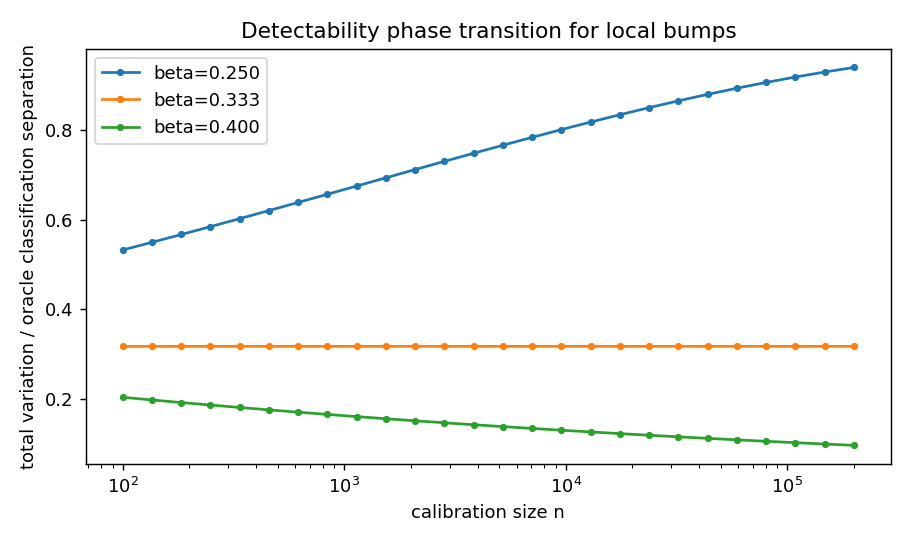
\includegraphics[width=0.62\textwidth]{fig_phase_transition.png}
\caption{Total variation between the two $n$-sample laws, for a bump bandwidth
$h=n^{-\beta}$. At the critical $\beta=1/(2s+d)=1/3$ it is flat at $0.317$. Below it rises
to one (detectable), above it falls to zero (invisible).}
\label{fig:phase}
\end{figure}

\begin{figure}[t]
\centering
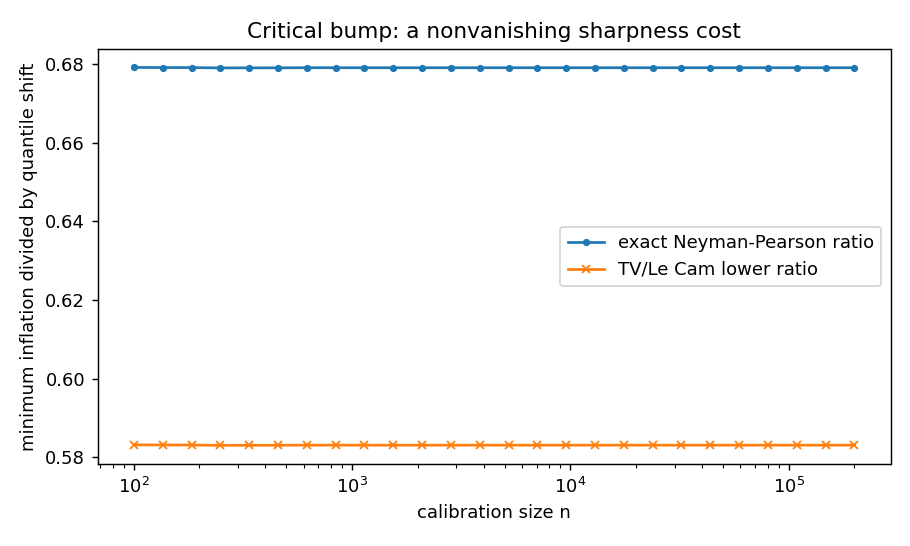
\includegraphics[width=0.62\textwidth]{fig_np_frontier.png}
\caption{Minimum inflation forced at the smooth baseline, as a fraction of the quantile
shift. The exact Neyman--Pearson frontier ($0.679$) sits well above the crude Le~Cam/TV
bound ($0.583$), and both are constant in $n$ and above $\tfrac12$.}
\label{fig:frontier}
\end{figure}

\begin{figure}[t]
\centering
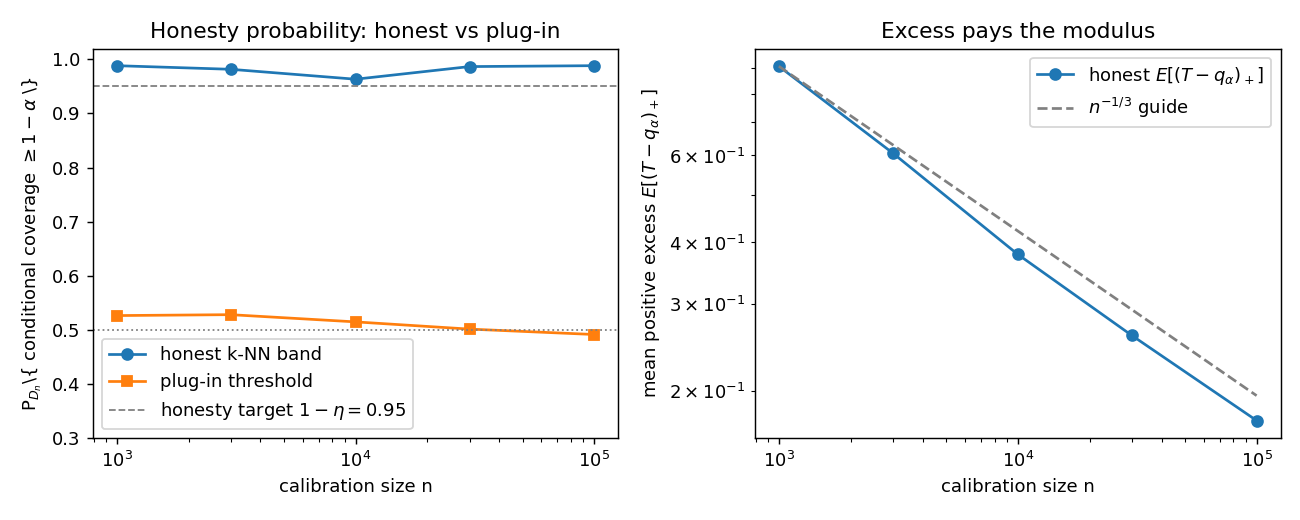
\includegraphics[width=0.62\textwidth]{fig_attainability.png}
\caption{Lognormal scores at the smooth baseline, $\eta=0.05$. Left: the honesty
probability, the probability over calibration samples that the realized threshold attains
conditional coverage at least $1-\alpha$. The honest $k$-nearest-neighbour band
\eqref{eq:knn} clears the target $1-\eta=0.95$. The uncorrected plug-in meets it on about
half the samples. Right: the honest band's positive excess $\E[(T-q_\alpha)_+]$, decaying at
the predicted $n^{-1/3}$.}
\label{fig:attain}
\end{figure}

\section{What it says for conformal prediction}

The obstruction is not exchangeability, weighting, or pooling. Localized conformal sets
that reweight by proximity are marginally valid and can be sharp. The obstruction is
indistinguishability under an honesty requirement. Three statements should be kept apart.
Zero or $o(r_n)$ oracle excess is incompatible with honesty. Minimax-rate sharpness,
$O(r_n)$ excess at a known smoothness $s$, is compatible with honesty \emph{for fixed
$\eta>0$}, and Section~\ref{sec:attain} attains it, and at $\eta=0$ even that fails
(Remark~\ref{rem:endpoint}). The smooth-class rate while honest over a rougher class is
again incompatible. Theorem~\ref{thm:main} is therefore a nonparametric \emph{inflation}
theorem, not a claim that honesty and minimax-rate sharpness never coexist, and
Theorem~\ref{thm:adapt} is the genuine separation.

The applied reading is the one experience already supplies. At small effective local sample
size $m_h$, the modulus $L h^{s} + m_h^{-1/2}$ is large and the honest set is inflated by a
correspondingly large amount. When the objective is a sharp predictive score rather than
high-probability local coverage, a kernel or local-likelihood estimate of the residual law
may be preferable, because it does not carry the one-sided insurance radius honesty
requires. Whether it wins is a separate decision-theoretic comparison under the chosen
score, not a corollary of the width bound. The honest guarantee is not free. A nontrivial
fixed-point honest guarantee requires structural assumptions on the conditional law.
Without them, distribution-free pointwise validity is generally vacuous. Its price is the
sharpness it surrenders to insure against the alternatives the data cannot rule out.

\bibliographystyle{plainnat}
\begin{thebibliography}{9}
\bibitem[Cai and Low(2004)]{cai2004adaptation} Cai, T.~T. and Low, M.~G. (2004). An
  adaptation theory for nonparametric confidence intervals. \emph{Annals of Statistics}
  32(5), 1805--1840.
\bibitem[Lei and Wasserman(2014)]{lei2014distribution} Lei, J. and Wasserman, L. (2014).
  Distribution-free prediction bands for non-parametric regression. \emph{Journal of the
  Royal Statistical Society, Series B} 76(1), 71--96.
\bibitem[Li(1989)]{li1989honest} Li, K.-C. (1989). Honest confidence regions for
  nonparametric regression. \emph{Annals of Statistics} 17(3), 1001--1008.
\bibitem[Low(1997)]{low1997nonparametric} Low, M.~G. (1997). On nonparametric confidence
  intervals. \emph{Annals of Statistics} 25(6), 2547--2554.
\bibitem[Tsybakov(2009)]{tsybakov2009introduction} Tsybakov, A.~B. (2009).
  \emph{Introduction to Nonparametric Estimation}. Springer.
\bibitem[Vovk(2012)]{vovk2012conditional} Vovk, V. (2012). Conditional validity of
  inductive conformal predictors. \emph{Proceedings of the Asian Conference on Machine
  Learning}, PMLR 25, 475--490.
\end{thebibliography}

\end{document}
